\documentclass[a4paper,11pt,french]{article}
\usepackage[utf8]{inputenc}

\usepackage[T1]{fontenc}
\usepackage[francais]{babel} 
\usepackage[top=2cm, bottom=2cm, left=2cm, right=2cm, includeheadfoot]{geometry} %pour les marges
\usepackage{lmodern}
\usepackage{pict2e}
\usepackage{fancyhdr} % Required for custom headers
\usepackage{lastpage} % Required to determine the last page for the footer
\usepackage{extramarks} % Required for headers and footers
\usepackage{graphicx} % Required to insert images
\usepackage{tabularx, longtable}
\usepackage{color, colortbl}
\usepackage{lscape}
%\usepackage[hidelinks]{hyperref}
\usepackage{longtable}
\usepackage{multirow}
\usepackage{rotating}
%\usepackage{pgfgantt}
%\usepackage{pgfcalendar}
%\usepackage{ifthen}
\usepackage{gensymb}

\linespread{1.1} % Line spacing

% Set up the header and footer
\pagestyle{fancy}
\lhead{\textbf{\hmwkClass -- \hmwkSubject \\ \hmwkTitle \\ \hmwkDocName}} % Top left header
\rhead{
\includegraphics[width=10em]{logo_univ.png}}
\lfoot{\lastxmark} % Bottom left footer
\cfoot{} % Bottom center footer
\rfoot{Page\ \thepage\ / \pageref{LastPage}} % Bottom right footer
\renewcommand\headrulewidth{0.4pt} % Size of the header rule
\renewcommand\footrulewidth{0.4pt} % Size of the footer rule

\setlength{\headheight}{40pt}

\newcommand{\hmwkTitle}{Transchiffrement} % Assignment title
\newcommand{\hmwkClass}{Master 2 SSI } % Course/class
\newcommand{\hmwkAuthorName}{Julien Bourdon} % Your name
\newcommand{\hmwkSubject}{Conduite de projet} % Subject
\newcommand{\hmwkDocName}{Spécification Technique du Besoin} % Document name

\newcommand{\version}{1.0} % Document version
\newcommand{\docDate}{27 novembre 2011} % Document date
\newcommand{\checked}{} % Checker name
\newcommand{\approved}{} % Approver name

\makeatletter
\newcommand{\resettranslate}{\let\translate\@firstofone}
\makeatother

\definecolor{gris}{rgb}{0.95, 0.95, 0.95}

\title{
\vspace{2in}
\textmd{\textbf{\hmwkClass :\ \hmwkTitle}}\\
\normalsize\vspace{0.1in}\small{Due\ on\ \hmwkDueDate}\\
\vspace{0.1in}\large{\textit{\hmwkClassInstructor\ \hmwkClassTime}}
\vspace{3in}
}

\author{\hmwkAuthorName}
\date{} % Insert date here if you want it to appear below your name


\usepackage{amsmath}
\begin{document}
\newcount\startdate
\newcount\daynum
%\pgfcalendardatetojulian{2013-01-021}{\startdate}
\pagestyle{fancy}

\vspace*{5cm}
\begin{center}\textbf{\Huge{\hmwkDocName}}\end{center}
\vspace*{4.5cm}
	

\fcolorbox{black}{gris}{
\begin{minipage}{15cm}
\begin{tabularx}{10cm}{lXl}
	\bfseries{Version} & & \version\\
	& & \\
	\bfseries{Date} & & \docDate\\
	& & \\
	\bfseries{Rédigé par} & & \hmwkAuthorName \\
	& & \\
	\bfseries{Relu par} & & \checked \\
	& & \\
	\bfseries{Approuvé par} & & \approved \\
	& & \\
\end{tabularx}
\end{minipage}
}

\newpage

%Tableau de mises à jour
\vspace*{1cm}
\begin{center}
\textbf{\huge{Versions}}\\
\vspace*{3cm}
	\begin{tabularx}{16cm}{|c|c|X|}
	\hline
	\bfseries{Version} & \bfseries{Date} & \bfseries{Modifications réalisées}\\
	\hline
	1.0 & 27/11/2013 & Création\\
	\hline
	1.1 & 20/01/2014 & Prise en compte des remarques suite aux réunions client et à l'audit.\\
	\hline
	\end{tabularx}
\end{center}

%La table des matières
\clearpage
\tableofcontents
\clearpage


\newpage
\section{Présentation de la mission du produit logiciel}


La première partie du projet est de créer un proxy transparent qui réalise du transchiffrement, c'est à dire de récupérer toutes les conversations normalement impossibles à lire entre un client et le serveur auquel il veut avoir accès.
Pour ce faire, il faut d'abord trouver un moyen d'authentifier notre proxy en utilisant une autorité de certification pour signer les certificats que nous allons créer par la suite.
Nous avons 3 choix qui s'offrent à nous :

\begin{itemize}
\item Installer directement notre autorité de certification dans le système.
\item Forcer l'utilisateur à accepter notre autorité de certification
\item Forger un faux certificat d'autorité qui a le même haché MD5 qu'un certificat d'autorité valide existant.
\end{itemize}

Cette dernière façon de faire étant plus compliquée à réaliser, nous allons en faire la deuxième partie de notre projet que nous détaillerons un peu plus loin.

Une fois l'autorité installée et acceptée, nous l'utiliserons pour signer des certificats correspondant aux serveurs auxquels le client veut se connecter que nous créerons à la volée. Une fois créés, nous pourrons les stocker pour une éventuelle réutilisation, ce qui nous fera gagner un temps précieux.

	Les connexions client / proxy et proxy / serveur seront soit en "clair" (HTTP) ce qui n'implique pas de transchiffrement car les données seront directement lisibles sur le réseau, soit chiffrées et de ce fait, notre proxy agira comme un « man in the middle ».

	La vitesse d'exécution est un facteur important pour ne pas que le proxy soit détecté pendant le déchiffrement / rechiffrement.

La deuxième partie du projet est surtout un travail de recherche sur les collisions MD5 afin de trouver un algorithme qui nous permette de forger cette fausse autorité. Nous aurons donc à faire tourner un programme de comparaison pendant une durée assez longue en parallèle de la première partie du projet.

\subsection{Terminologie et sigles utilisés}

\begin{description}
\item[Client] Utilisateur d'une machine privée (ordinateur) qui souhaite se connecter à un serveur web.
\item[Proxy] Machine intermédiaire écoutant sur le réseau qui va réaliser le transchiffrement TLS/SSL.
\item[Serveur] Serveur web, accessible à partir d'une URL.
\item[Autorité de certification] Ici, l'autorité utilise sa clé privée pour signer des certificats qui prouvent l'appartenance d'une clé publique à un individu.

\end{description}

\subsection{Liste des cas d'utilisation}

Pour commencer le projet, une liste des différents cas possibles d’utilisation de l’application a été faite afin de répondre au besoin du client selon leur priorité. Chaque cas est alors développé afin d’identifier les étapes nécessaires pour sa réalisation. 

\begin{center}
\begin{tabular}{|c|c|c|}
\hline 
ID & Intitulé & Priorité \\ 
\hline 
P.1 & Configuration du proxy  & Indispensable \\ 
\hline 
P.2 & Installation de l'autorité & Indispensable \\ 
\hline 
P.3 & Acceptation de l'autorité & Optionnel \\ 
\hline 
P.4 & Génération de certificats & Indispensable \\ 
\hline 
P.5 & Transchiffrement & Indispensable \\ 
\hline 
P.6 & Forge d'une fausse autorité & Optionnel \\ 
\hline 
\end{tabular} 
\end{center}
~~\\
~~\\

\huge
\subsection{Diagramme UML}
\begin{center}
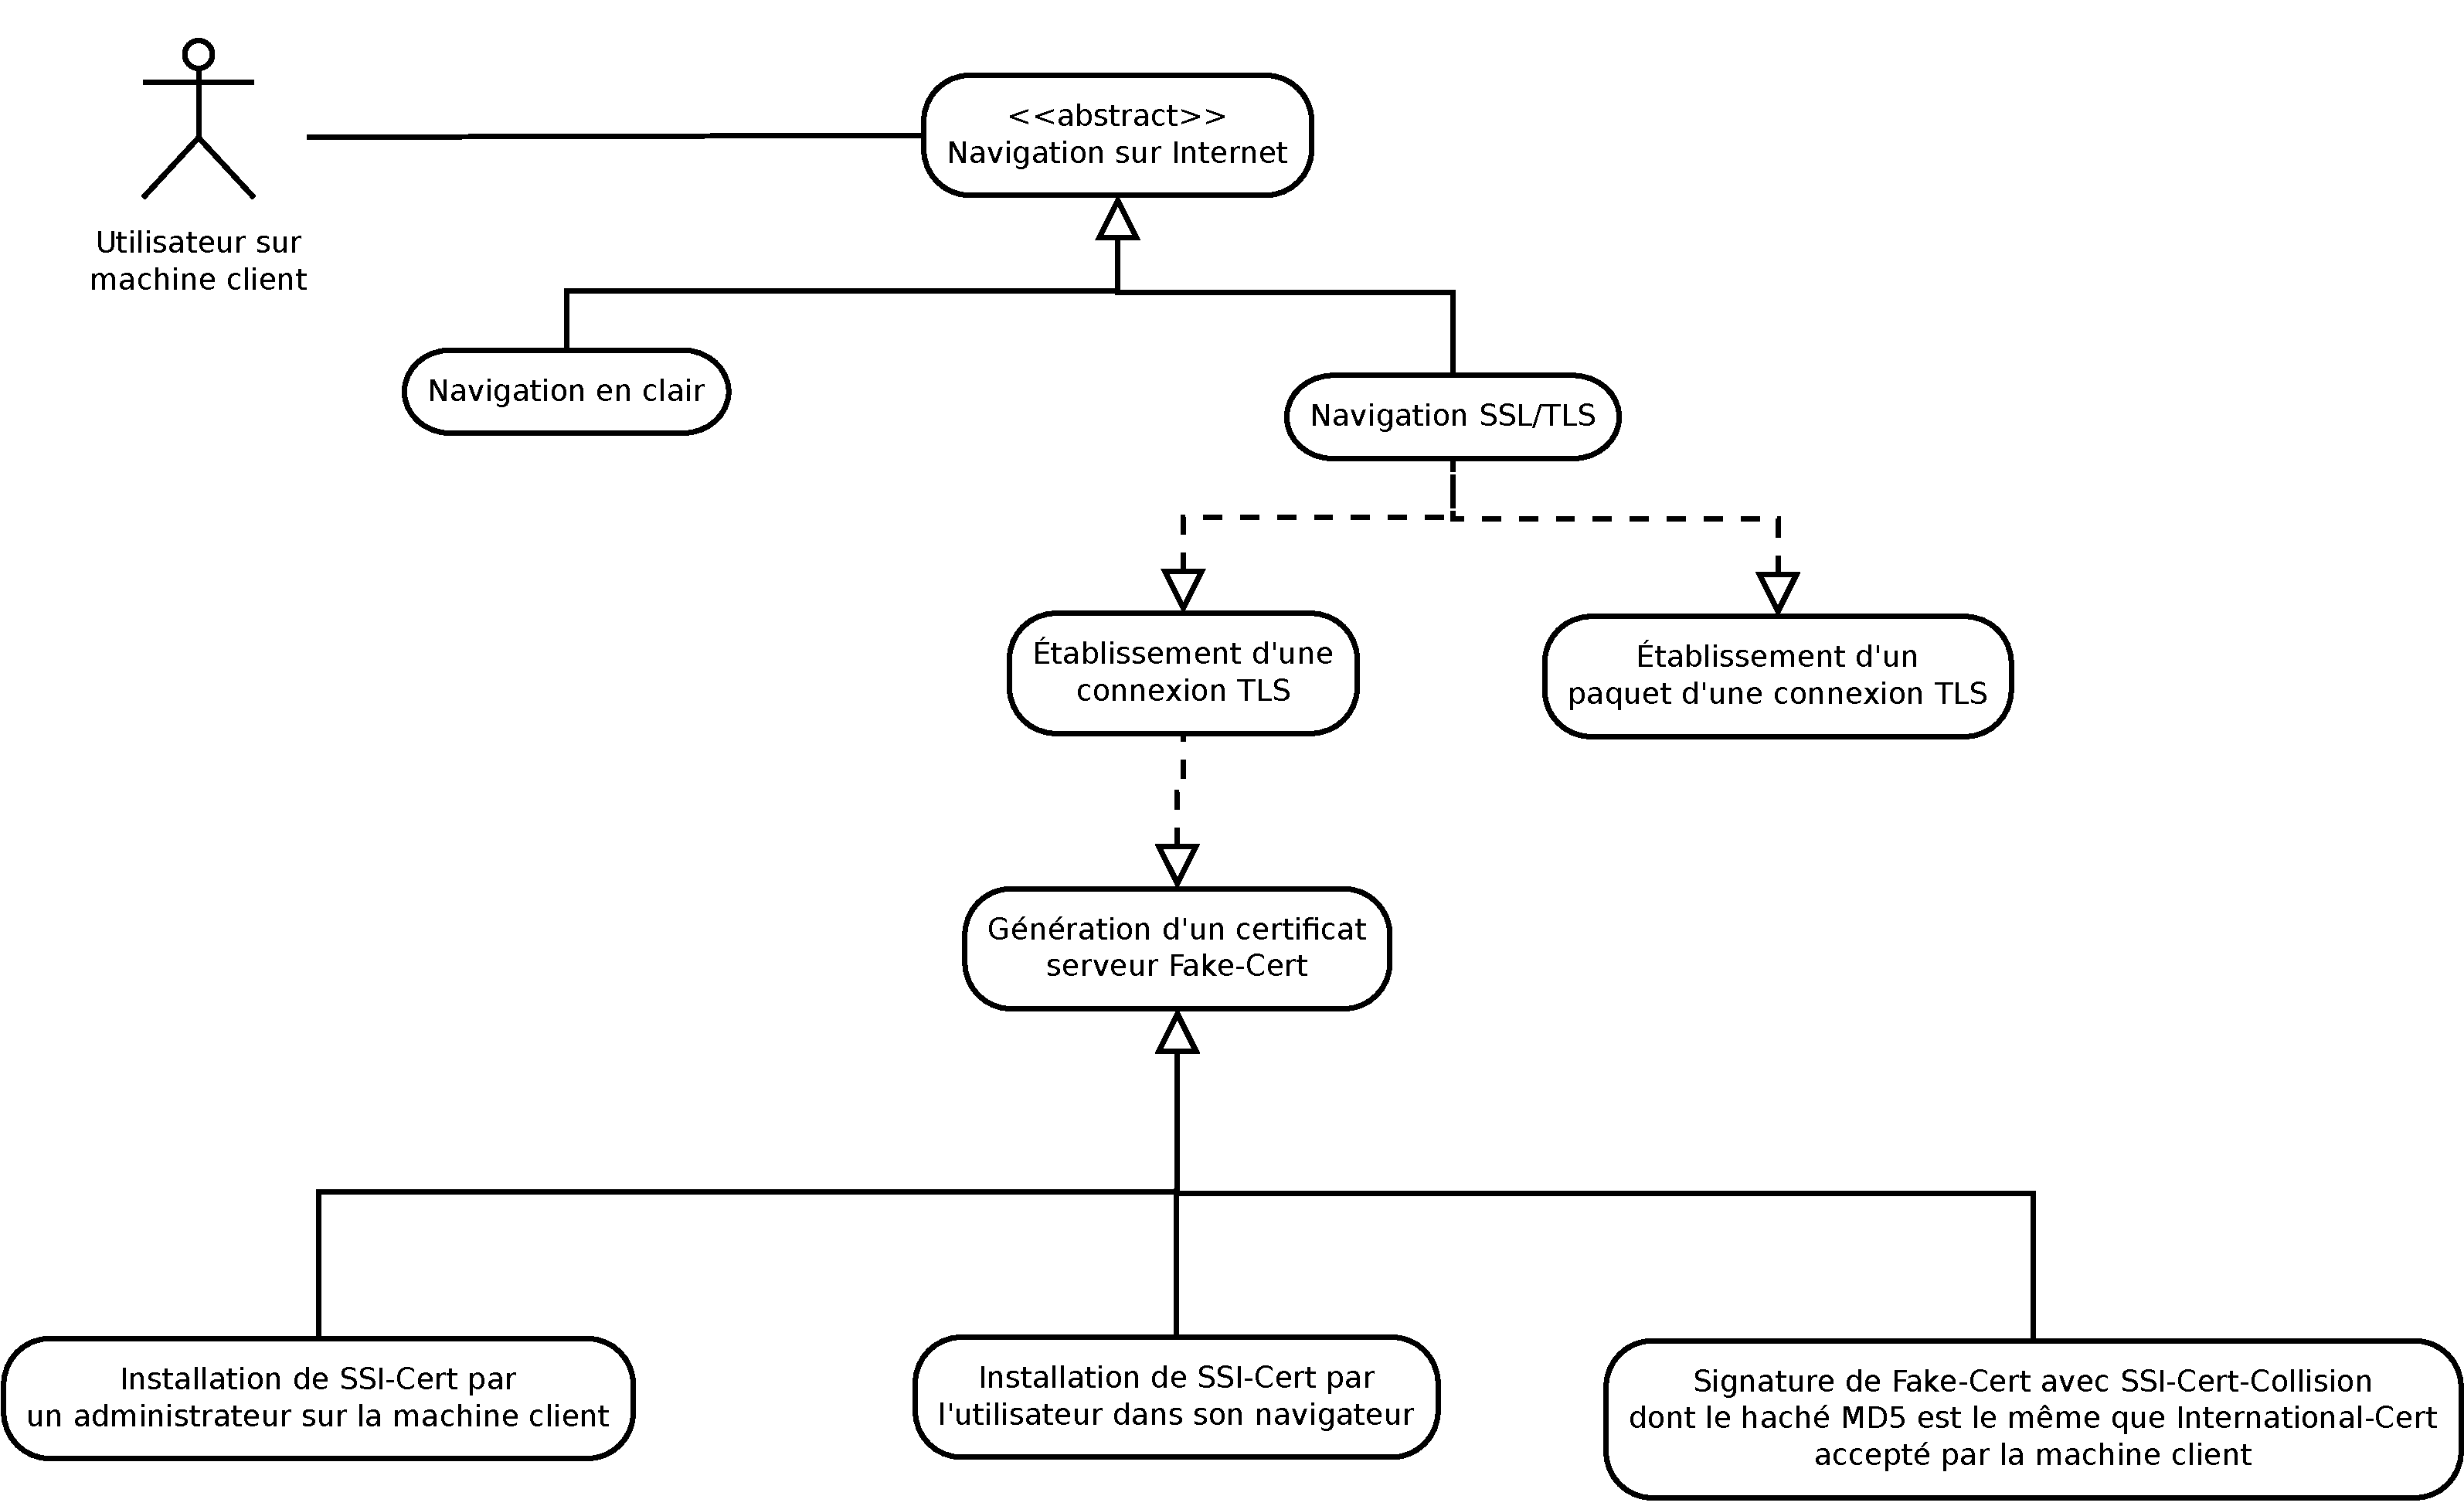
\includegraphics[width=\textwidth]{images/cas_utilisation.pdf}
\end{center}
\normalsize

\subsection{Schémas explicatifs}

\subsubsection{Phase de partage de certificats}

\begin{center}
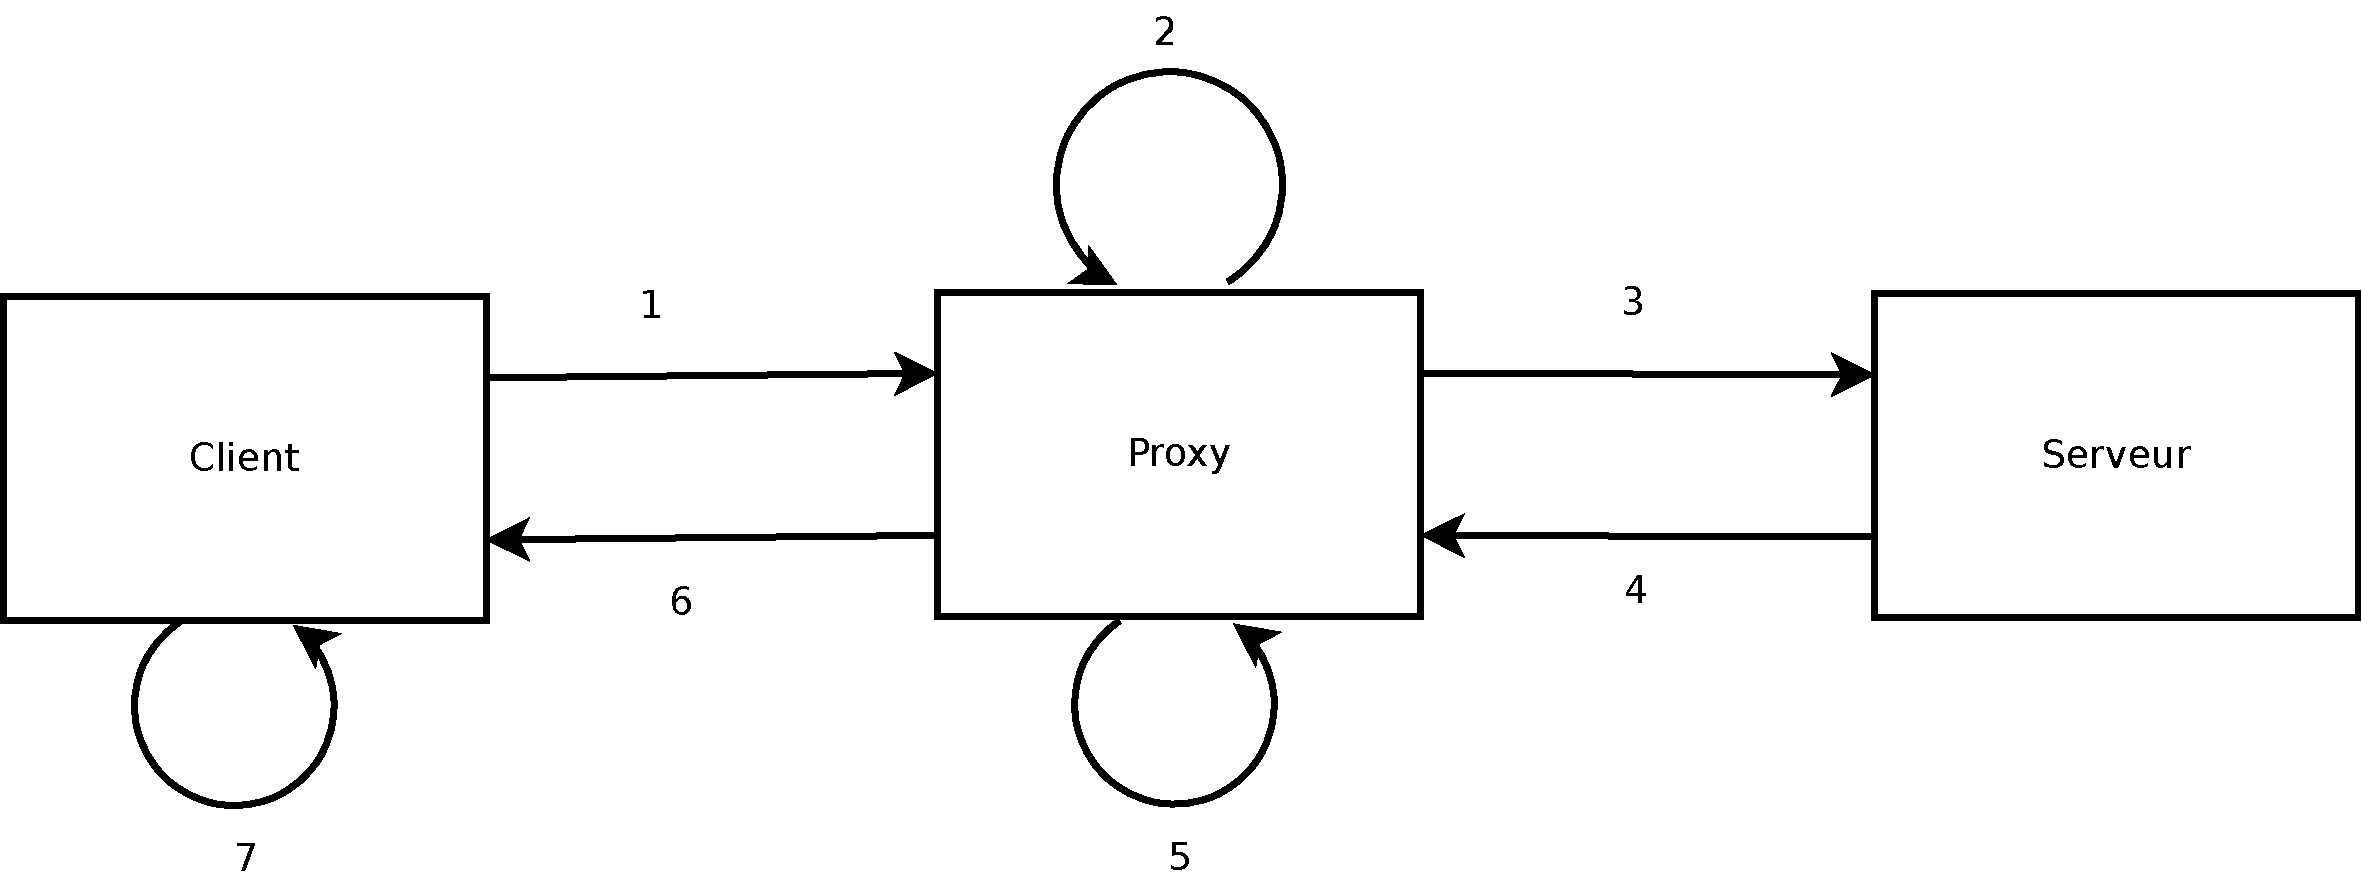
\includegraphics[width=\textwidth]{images/Certificats.pdf}
\end{center}

1. Le client envoie une requête au serveur pour négocier une connexion SSL/TLS.

2. Le proxy intercepte la requête.

3. Le proxy envoie sa propre requête de connexion au serveur demandé par le client.

4. Le serveur répond au proxy et envoie son certificat signé par une autorité.

5. Le proxy génère un faux certificat avec la clé publique du proxy et la signature de notre autorité.

6. Le proxy envoie le faux certificat au client.

7. Le client vérifie que le certificat est valide.\\

Une fois les certificats partagés, il faut maintenant échanger une clé de session pour avoir une connexion sécurisée.

\subsubsection{Phase d'échange des clés}

\begin{center}
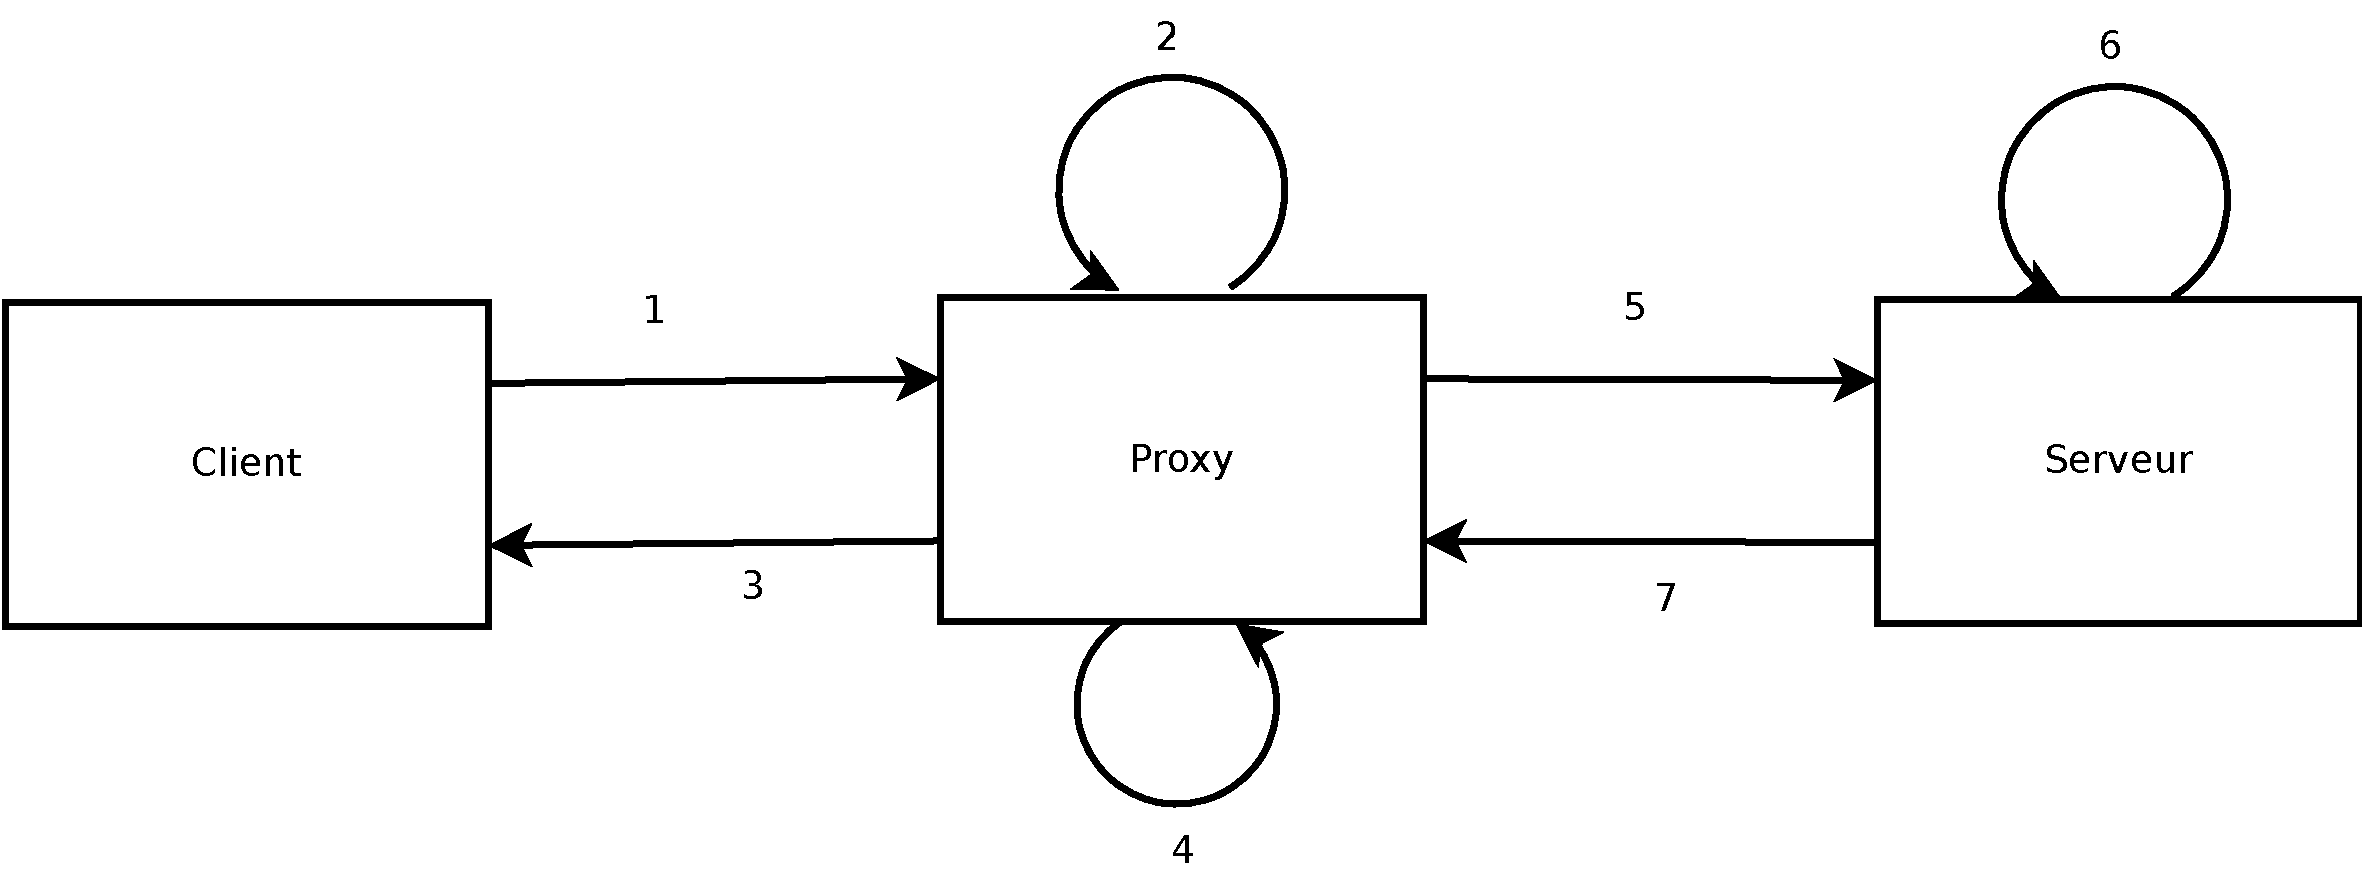
\includegraphics[width=\textwidth]{images/Cles.pdf}
\end{center}


1. Le client envoie une clé de session chiffrée avec la clé publique présente sur le certificat du proxy.

2. Le proxy déchiffre avec la clé privée associée.

3. Le proxy ouvre une connexion sécurisée avec le client avec la clé de session.

4. Le proxy chiffre une nouvelle clé de session avec la clé publique du serveur.

5. Le proxy envoie la clé chiffrée au serveur.

6. Le serveur déchiffre la clé de session.

7. Le serveur ouvre une connexion sécurisée avec le proxy en utilisant la clé de session.


\section{Cas d'utilisation}

\subsection{Configuration du proxy}

Installation et configuration du proxy pour que tout le trafic en provenance du client passe par le proxy.

\begin{tabular}{|>{\columncolor[gray]{.8}}m{4cm}|m{12cm}|}
   \hline
   Description & Mise en place du proxy \\
   \hline
   Pré-conditions & Implémentation du cas d'utilisation Transchiffrement\\
   \hline
   Évènement déclenchant & Début du projet \\
   \hline
   Condition d'arrêt & Proxy installé \\
   \hline
   Cas d'exception  &  \\
   \hline   
\end{tabular}

~\\

Description du flot d'évènements principal :

\begin{tabular}{|m{8cm}|m{8cm}|}
   \hline
   Acteur(s) & Système \\
   \hline
   1. Lancement de l'exécutable du proxy & \\
   \hline
\end{tabular}

\subsection{Installation de l'autorité}

Dans ce cas de figure, on prend l'exemple d'un administrateur système qui installe directement l'autorité sur les machines clientes.

\begin{tabular}{|>{\columncolor[gray]{.8}}m{4cm}|m{12cm}|}

   \hline
   Description & Première façon de faire : installer directement l'autorité dans le système\\
   \hline
   Pré-conditions &Autorité par défaut présente \\
   \hline
   Évènement déclenchant &  Mise en place de l'autorité\\
   \hline
   Condition d'arrêt & Autorité reconnue comme valide \\
   \hline
   Cas d'exception  & \\
   \hline   
\end{tabular}


~\\

Description du flot d'évènements principal :

\begin{tabular}{|m{8cm}|m{8cm}|}
   \hline
   Acteur(s) & Système \\
   \hline
   1. Installation de l'autorité directement dans le système du client. & \\
   \hline
\end{tabular}

\subsection{Acceptation de l'autorité}

Dans ce cas de figure, on veut forcer le client à accepter notre fausse autorité par une suite d'actions de paramétrage dans son navigateur.

\begin{tabular}{|>{\columncolor[gray]{.8}}m{4cm}|m{12cm}|}
   \hline
   Description & Deuxième façon de faire : faire accepter au client notre autorité.\\
   \hline
   Pré-conditions & Pas d'autorité présente\\
   \hline
   Évènement déclenchant & Première connexion au proxy par le client \\
   \hline
   Condition d'arrêt & Autorité reconnue comme valide \\
   \hline
   Cas d'exception  & L'autorité n'est pas acceptée par le client. \\
   \hline   
\end{tabular}

~\\

Description du flot d'évènements principal :

\begin{tabular}{|m{8cm}|m{8cm}|}
   \hline
  \rowcolor[gray]{.8} Acteur(s) & Système \\
   \hline
   1. Le client se connecte au proxy. & \\
   \hline
    & 2. Proposition de l'autorité au client. \\
   \hline
   3. Le client accepte et installe l'autorité. &  \\
   \hline
\end{tabular}


\subsection{Utilisation d'une fausse autorité forgée}

Si la deuxième partie du projet a donné un résultat, nous aurons donc réussi à forger un faux certificat d'autorité ayant le même haché MD5 que celui choisi.
Dans ce cas, nous utiliserons ce certificat.

\begin{tabular}{|>{\columncolor[gray]{.8}}m{4cm}|m{12cm}|}
   \hline
   Description & Utilisation d'une fausse autorité forgée \\
   \hline
   Pré-conditions & L'algorithme de recherche a renvoyé un certificat ayant le même haché MD5 que celui attendu.
 \\
   \hline
   Évènement déclenchant & L'algorithme de recherche a donné une réponse positive \\
   \hline
   Condition d'arrêt & L'autorité est reconnue comme valide \\
   \hline
   Cas d'exception  &  L'algorithme de recherche n'a pas donné le résultat voulu et nous n'utiliserons pas cette  façon de faire. \\
   \hline   
\end{tabular}

~\\

~\\

Description du flot d'évènements principal :

\begin{tabular}{|m{8cm}|m{8cm}|}
   \hline
  \rowcolor[gray]{.8} Acteur(s) & Système \\
   \hline
   1. Le client se connecte au proxy. & \\
   \hline
    & 2. Proposition de l'autorité au client. \\
   \hline
      3. Le client compare les hachés MD5 des deux autorités et l'accepte car ils sont égaux & \\
   \hline
    4. Le client installe l'autorité. &  \\
   \hline
\end{tabular}

\subsection{Génération de certificats}

Une fois l'autorité acceptée, à chaque demande de connexion HTTPS du client à un serveur, un faux certificat doit être généré à la volée.

\begin{tabular}{|>{\columncolor[gray]{.8}}m{4cm}|m{12cm}|}
   \hline
   Description & Génération d'un faux certificat pour le serveur \\
   \hline
   Pré-conditions & Le client ne s'est pas encore connecté à ce serveur \\
   \hline
   Évènement déclenchant & Le client tente de se connecter à un serveur \\
   \hline
   Condition d'arrêt &  Certificat généré et valide \\
   \hline
   Cas d'exception  &  Si le client s'est déjà connecté à ce serveur, on va le chercher dans une liste de certificats déjà générés auparavant.
\\
   \hline   
\end{tabular}

~\\

Description du flot d'évènements principal :

\begin{tabular}{|m{8cm}|m{8cm}|}
   \hline
  \rowcolor[gray]{.8} Acteur(s) & Système \\
   \hline
   1. Le client tente de se connecter à un serveur & \\
   \hline
    & 
2. Un faux certificat semblable en tout point au vrai est généré, seule la clé publique est remplacée par celle du proxy \\
   \hline
\end{tabular}

\subsection{Transchiffrement des paquets d'une connexion HTTPS}

Une fois le certificat généré, le client établit une connexion TLS/SSL et envoie sa requête au proxy de manière chiffrée, le proxy déchiffre, la garde dans les logs (éventuellement) puis rechiffre cette requête pour le serveur (avec une autre clé). Le but de ce processus est d'être transparent donc très rapide.
On a bien évidemment le même processus dans l'autre sens pour la réponse du serveur au client.

\begin{tabular}{|>{\columncolor[gray]{.8}}m{4cm}|m{12cm}|}
   \hline
   Description & Déchiffrement / Rechiffrement de la requête du client pour l'envoyer au serveur et de la réponse du serveur pour l'envoyer au client. \\
   \hline
   Pré-conditions & Certificat généré et deux connexions TLS/SSL ouvertes\\
   \hline
   Évènement déclenchant &  Envoi d'une requête du client\\
   \hline
   Condition d'arrêt & Message rédigé et transfert d’envoi terminé \\
   \hline
   Cas d'exception  & Renégociation TLS/SSL \\
   \hline   
\end{tabular}

~\\

Description du flot d'évènements principal :

\begin{tabular}{|m{8cm}|m{8cm}|}
   \hline
  \rowcolor[gray]{.8} Acteur(s) & Système \\
   \hline
   1. Envoi d'une requête chiffrée par le client & \\
   \hline
    &
2. Déchiffrement de la requête

3. Log de cette requête

4. Rechiffrement de la requête pour le serveur

5. Envoi de cette requête au serveur


8. Réception de la réponse chiffrée

9. Déchiffrement de la réponse

10. Log de la réponse

11. Rechiffrement de la réponse

12. Envoi de la réponse au client \\
   \hline
  6. Traitement de la requête par le serveur
  
7. Envoi de la réponse au proxy  &  \\
   \hline
\end{tabular}

\subsection{Transfert des paquets HTTP}

Si le client tente de se connecter en HTTP à un serveur web, on ne fait que de transférer les paquets.

\begin{tabular}{|>{\columncolor[gray]{.8}}m{4cm}|m{12cm}|}
   \hline
   Description & Transfert des paquets en clair \\
   \hline
   Pré-conditions & Proxy configuré pour le HTTP\\
   \hline
   Évènement déclenchant &  Envoi d'une requête du client\\
   \hline
   Condition d'arrêt & Message rédigé et transfert d’envoi terminé \\
   \hline
   Cas d'exception  & \\
   \hline   
\end{tabular}

~\\

Description du flot d'évènements principal :

\begin{tabular}{|m{8cm}|m{8cm}|}
   \hline
  \rowcolor[gray]{.8} Acteur(s) & Système \\
   \hline
   1. Envoi d'une requête en clair par le client & \\
   \hline
& 2. Transfert de la requête au serveur  \\
& 3. Réception de la réponse du serveur  \\
   \hline
  
4. Envoi de la réponse au client  &  \\
   \hline
\end{tabular}

\section{Etude}

Notre étude porte sur la recherche de seconde pré-image du MD5.\\
Nous devons comprendre le fonctionnement de MD5 et utiliser la faiblesse de cet algorithme.\\
Nous allons développer un algorithme de recherche pour générer un certificat d'autorité ayant le même haché qu'un existant choisi.\\
Nous savons que le champ qui permet le plus de modifications est celui de la clé publique du certificat.\\
Grâce à une étude réalisée en 2008, nous savons quels champs nous pouvons modifier pour que le haché MD5 soit le plus proche de l'original.\\
C'est donc sur les bits du modulo de la clé publique que nous allons opérer la majeure partie des changements.\\
Pour que ce certificat d'autorité soit considéré comme valide, il faut que le haché de ce certificat soit le même que celui que nous voulons imiter.\\
Si nous arrivons à générer un certificat d'autorité remplissant cette condition, nous pourrons l'inclure dans le proxy de transchiffrement.\\
Nous serons donc capables de signer les certificats générés à la volée quand un utilisateur veut y avoir accès.\\
Grâce à ces faux-certificats, nous pourrons alors voir tout ce qui transite sans que l'utilisateur s'en aperçoive.\\
Nous allons donc livrer un rapport d'étude pour expliquer notre démarche pour la création de l'algorithme.\\

\section{Performances}
Pour que notre proxy soit considéré comme "transparent", nous devons remplir des contraintes de temps d'exécution du transchiffrement.
On s'autorise donc une seconde de marge pour toute page générée très rapidement et jusqu'à 200\% du temps pour une page contenant un volume conséquent de données.

\end{document}